\documentclass[10pt]{article}

\usepackage[margin=1in]{geometry}
\usepackage{amsmath}
\usepackage{booktabs}
\usepackage{graphicx}
\usepackage{hyperref}
\usepackage{microtype}
\usepackage{subcaption}
\usepackage{tikz}
\usepackage{pgfplots}
\usetikzlibrary{arrows.meta,positioning,shapes.geometric}
\pgfplotsset{compat=1.18}

\title{Bringing Qwen3.5-0.8B Vision-Language Inference to MLC LLM: \\
An Engineering Report on Model Support, Correctness, and Batch-1 Performance}

\author{
  Familiar AI Engineering Notes \\
  \texttt{familiar-ai/logos-multitask-qwen3.5-2026-05-03-best}
}

\date{May 2026}

\begin{document}
\maketitle

\begin{abstract}
We report on an implementation effort that added support for a fine-tuned
Qwen3.5 0.8B vision-language model in MLC LLM. The work covered model
configuration, tokenizer and image preprocessing parity, a vision tower,
multi-rope positional handling, mixed full-attention and linear-attention
decoder layers, Gated DeltaNet state management, weight conversion, MLC model
library compilation, and apples-to-apples benchmarking against Transformers and
vLLM. The resulting CUDA artifact runs the Familiar AI checkpoint on a
single-image batch-1 workload with the same image grid and generated-token
count as the vLLM baseline. On the Kentucky image prompt with 128 generated
tokens, the current MLC path measured 414.23 generated tokens/s and 446.09
effective decode tokens/s, while the vLLM path measured 413.30 generated
tokens/s. This report is not a claim of general serving superiority; instead,
it is an arXiv-style engineering paper that records the design, validation
methodology, performance trajectory, diagrams, and lessons learned from bringing
one non-standard multimodal architecture to a machine-learning compiler stack.
\end{abstract}

\section{Introduction}

Large language model deployment is no longer a matter of compiling a single
Transformer block. Modern checkpoints combine custom tokenizers, image or audio
front-ends, grouped-query attention, hybrid state-space or linear-attention
layers, rotary variants, and runtime-specific cache formats. Compiler-based
systems such as TVM and MLC LLM promise portability and aggressive
specialization, but that promise is tested most sharply by non-standard model
families whose inference semantics do not already match common LLaMA-style
templates.

This paper documents the work required to support a fine-tuned Familiar AI
Qwen3.5 0.8B vision-language checkpoint in MLC LLM. The model uses a vision
tower, multimodal rotary position handling, 24 language layers, a repeated
pattern of Gated DeltaNet linear-attention layers and full-attention layers, and
a large vocabulary. The deployment target studied here is deliberately narrow:
single-GPU CUDA, batch size 1, one image, and fixed-token generation. This
setting was chosen because it is small enough to diagnose precisely and
important enough to expose the interaction between model semantics, compiler
lowering, external kernels, and runtime scheduling.

\begin{figure}[t]
  \centering
  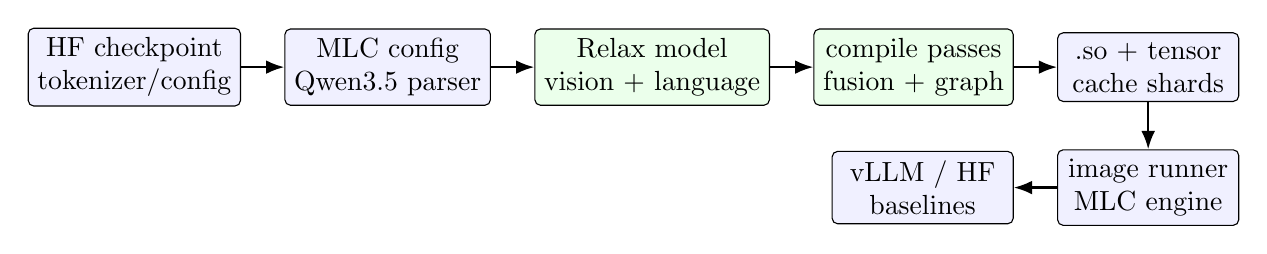
\begin{tikzpicture}[
    box/.style={draw, rounded corners=2pt, align=center, minimum height=0.72cm, minimum width=2.3cm, fill=blue!6},
    opt/.style={draw, rounded corners=2pt, align=center, minimum height=0.72cm, minimum width=2.3cm, fill=green!8},
    arrow/.style={-Latex, thick}
]
\node[box] (hf) {HF checkpoint\\tokenizer/config};
\node[box, right=0.55cm of hf] (config) {MLC config\\Qwen3.5 parser};
\node[opt, right=0.55cm of config] (model) {Relax model\\vision + language};
\node[opt, right=0.55cm of model] (passes) {compile passes\\fusion + graph};
\node[box, right=0.55cm of passes] (runtime) {.so + tensor\\cache shards};
\node[box, below=0.6cm of runtime] (serve) {image runner\\MLC engine};
\node[box, left=0.55cm of serve] (compare) {vLLM / HF\\baselines};
\draw[arrow] (hf) -- (config);
\draw[arrow] (config) -- (model);
\draw[arrow] (model) -- (passes);
\draw[arrow] (passes) -- (runtime);
\draw[arrow] (runtime) -- (serve);
\draw[arrow] (serve) -- (compare);
\end{tikzpicture}

  \caption{End-to-end path from Hugging Face checkpoint to MLC model library and
  benchmark comparison.}
  \label{fig:pipeline}
\end{figure}

The central result is parity with a vLLM baseline on the same model and image
preprocessing path. The result emerged less from a single optimization than
from a sequence of correctness and systems changes: image grid parity,
configuration handling, safe weight remapping, Gated DeltaNet support, stable
decode inputs, explicit paged metadata, CUDA graph capture, and robust
benchmarking. Figure~\ref{fig:pipeline} sketches the resulting workflow.

\section{Background}

\paragraph{MLC LLM and TVM.}
MLC LLM builds on TVM's compiler stack, which lowers high-level model programs
to optimized target-specific code through graph-level and tensor-level
transformations~\cite{chen2018tvm}. In the deployment studied here, MLC exports
model functions such as image embedding, multimodal prefill, and multimodal
decode into a compiled CUDA shared library and a parameter shard directory.

\paragraph{vLLM.}
vLLM is a high-throughput LLM serving system best known for PagedAttention,
which manages KV cache memory in blocks and decouples logical sequence layout
from physical allocation~\cite{kwon2023pagedattention}. It is the relevant
competitor for this work because it is optimized for online decoding and
already supports modern attention backends and CUDA graph reuse.

\paragraph{FlashInfer.}
FlashInfer provides optimized and customizable inference kernels for attention
and related LLM serving operations~\cite{flashinfer2025}. In the MLC artifact
described here, FlashInfer is used for full-attention paths while cuBLAS handles
many projection and LM-head matrix-vector operations.

\section{Model Support}

The Familiar AI checkpoint used in this study is a fine-tuned Qwen3.5
vision-language model. The implementation had to represent both the vision
front-end and the language stack in MLC's Python model frontend.

\subsection{Configuration}

The language model has hidden size 1024, 24 decoder layers, 8 attention heads,
2 key-value heads for full attention, head dimension 256, and vocabulary size
248320. The benchmark artifact uses context window 2048, prefill chunk size
320, batch size 1, and unquantized fp16 weights with bf16 model compute where
configured. The model contains 852,985,920 parameters and converted weights
occupy approximately 1.589 GB.

\begin{figure}[t]
  \centering
  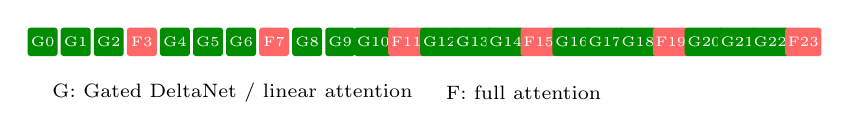
\begin{tikzpicture}[
    layer/.style={rectangle, rounded corners=1pt, minimum width=0.38cm, minimum height=0.36cm, text=white, inner sep=1pt}
]
\node[layer, fill=green!55!black] at (0.0,0) {\tiny G0};
\node[layer, fill=green!55!black] at (0.42,0) {\tiny G1};
\node[layer, fill=green!55!black] at (0.84,0) {\tiny G2};
\node[layer, fill=red!60] at (1.26,0) {\tiny F3};
\node[layer, fill=green!55!black] at (1.68,0) {\tiny G4};
\node[layer, fill=green!55!black] at (2.1,0) {\tiny G5};
\node[layer, fill=green!55!black] at (2.52,0) {\tiny G6};
\node[layer, fill=red!60] at (2.94,0) {\tiny F7};
\node[layer, fill=green!55!black] at (3.36,0) {\tiny G8};
\node[layer, fill=green!55!black] at (3.78,0) {\tiny G9};
\node[layer, fill=green!55!black] at (4.2,0) {\tiny G10};
\node[layer, fill=red!60] at (4.62,0) {\tiny F11};
\node[layer, fill=green!55!black] at (5.04,0) {\tiny G12};
\node[layer, fill=green!55!black] at (5.46,0) {\tiny G13};
\node[layer, fill=green!55!black] at (5.88,0) {\tiny G14};
\node[layer, fill=red!60] at (6.3,0) {\tiny F15};
\node[layer, fill=green!55!black] at (6.72,0) {\tiny G16};
\node[layer, fill=green!55!black] at (7.14,0) {\tiny G17};
\node[layer, fill=green!55!black] at (7.56,0) {\tiny G18};
\node[layer, fill=red!60] at (7.9799999999999995,0) {\tiny F19};
\node[layer, fill=green!55!black] at (8.4,0) {\tiny G20};
\node[layer, fill=green!55!black] at (8.82,0) {\tiny G21};
\node[layer, fill=green!55!black] at (9.24,0) {\tiny G22};
\node[layer, fill=red!60] at (9.66,0) {\tiny F23};
\node[anchor=west] at (0,-0.65) {\scriptsize G: Gated DeltaNet / linear attention};
\node[anchor=west] at (5.0,-0.65) {\scriptsize F: full attention};
\end{tikzpicture}

  \caption{Layer pattern in the 24-layer language stack. Every fourth layer is
  full attention; the remaining layers use a Gated DeltaNet linear-attention
  block.}
  \label{fig:model-structure}
\end{figure}

\subsection{Vision-Language Path}

The image path resizes the input to a fixed 512 by 512 canvas for the benchmark,
producing a grid of $(1,32,32)$ before spatial merge. The vision tower embeds
1024 patches and the merger produces 256 image tokens for the language model.
The MLC, Transformers, and vLLM paths were checked to use matching image-grid
metadata before reporting performance comparisons.

\begin{figure}[t]
  \centering
  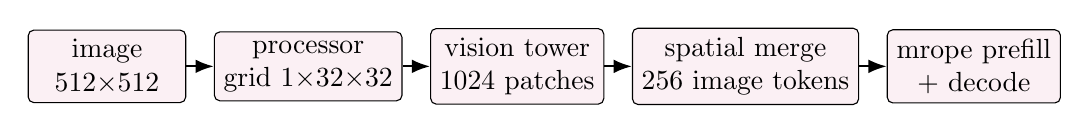
\begin{tikzpicture}[
    box/.style={draw, rounded corners=2pt, align=center, minimum height=0.68cm, minimum width=2.0cm, fill=purple!6},
    arrow/.style={-Latex, thick}
]
\node[box] (img) {image\\512$\times$512};
\node[box, right=0.35cm of img] (proc) {processor\\grid 1$\times$32$\times$32};
\node[box, right=0.35cm of proc] (vision) {vision tower\\1024 patches};
\node[box, right=0.35cm of vision] (merge) {spatial merge\\256 image tokens};
\node[box, right=0.35cm of merge] (lm) {mrope prefill\\+ decode};
\draw[arrow] (img) -- (proc);
\draw[arrow] (proc) -- (vision);
\draw[arrow] (vision) -- (merge);
\draw[arrow] (merge) -- (lm);
\end{tikzpicture}

  \caption{Image embedding path used in the benchmark. Matching the
  $1 \times 32 \times 32$ grid across MLC, Transformers, and vLLM was a
  prerequisite for apples-to-apples comparison.}
  \label{fig:image-path}
\end{figure}

\subsection{Hybrid Decoder}

The language stack alternates mostly linear-attention layers with sparse
full-attention layers. Figure~\ref{fig:model-structure} shows the exact pattern:
18 Gated DeltaNet layers and 6 full-attention layers. Supporting this stack
required a state object for recurrent linear attention, convolution state for
the Gated DeltaNet block, multimodal RoPE handling, and separate full-attention
KV cache behavior.

\begin{table}[t]
  \centering
  \caption{Selected model and compile-time parameters for the current artifact.}
  \label{tab:model-config}
  \begin{tabular}{ll}
    \toprule
    Parameter & Value \\
    \midrule
    Checkpoint & \texttt{familiar-ai/logos-multitask-qwen3.5-2026-05-03-best} \\
    Hidden size & 1024 \\
    Decoder layers & 24 \\
    Full-attention layers & 6 \\
    Linear-attention layers & 18 \\
    Attention heads / KV heads & 8 / 2 \\
    Head dimension & 256 \\
    Vocabulary size & 248320 \\
    Active vocabulary size & 248077 \\
    Context window & 2048 \\
    Prefill chunk size & 320 \\
    Batch size & 1 \\
    Parameter count & 852,985,920 \\
    Converted parameter size & 1.589 GB \\
    \bottomrule
  \end{tabular}
\end{table}

\section{Compiler and Runtime Integration}

\subsection{Exported Model Functions}

The final model exports an image embedding function, multimodal prefill
functions, and multimodal decode functions. For serving, the relevant hot path
is \texttt{decode\_mrope}, which consumes a one-token embedding, the paged KV
cache, recurrent state, and multimodal position metadata.

\subsection{Weight Conversion}

The source checkpoint uses Hugging Face safetensors. Conversion maps the model
weights into MLC tensor-cache shards, rewrites active vocabulary metadata from
the tokenizer, and preserves tokenizer files in the MLC model directory. A
separate vLLM preparation helper remaps selected parameter names so the same
fine-tuned checkpoint can be loaded in the installed vLLM environment.

\subsection{CUDA Graph Capture}

The largest runtime change was making decode replay stable under CUDA graph
capture. Earlier versions left multiple KV-cache append, metadata, and
cross-attention calls outside the graph or produced incorrect text when
capturing unsafe FlashInfer state. The final artifact uses explicit paged
metadata, stable decode inputs, and relaxed metadata-tuple analysis in the CUDA
graph rewrite pass. The resulting \texttt{decode\_mrope} path is captured as a
single graph replay per token.

\begin{figure}[t]
  \centering
  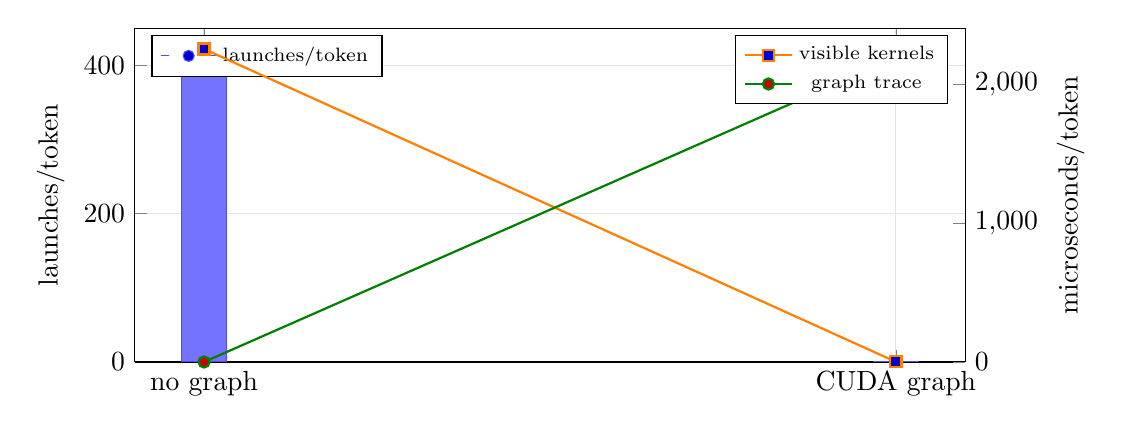
\begin{tikzpicture}
\begin{axis}[
    width=\linewidth,
    height=0.48\linewidth,
    ymin=0,
    ymax=450,
    ylabel={launches/token},
    symbolic x coords={no graph,CUDA graph},
    xtick=data,
    axis y line*=left,
    grid=major,
    major grid style={draw=black!10},
    legend style={at={(0.02,0.98)},anchor=north west,font=\scriptsize},
]
\addplot+[ybar, bar width=16pt, fill=blue!55, draw=blue!70] coordinates {
    (no graph,415.0)
    (CUDA graph,1.0)
};
\addlegendentry{launches/token}
\end{axis}
\begin{axis}[
    width=\linewidth,
    height=0.48\linewidth,
    ymin=0,
    ymax=2400,
    axis y line*=right,
    axis x line=none,
    ylabel={microseconds/token},
    symbolic x coords={no graph,CUDA graph},
    xtick=data,
    legend style={at={(0.98,0.98)},anchor=north east,font=\scriptsize},
]
\addplot+[mark=square*, thick, orange] coordinates {
    (no graph,2250.376)
    (CUDA graph,0.978)
};
\addlegendentry{visible kernels}
\addplot+[mark=*, thick, green!50!black] coordinates {
    (no graph,0.0)
    (CUDA graph,2189.405)
};
\addlegendentry{graph trace}
\end{axis}
\end{tikzpicture}

  \caption{CUDA graph capture changes the visibility of runtime work. With graph
  disabled, Nsight sees hundreds of kernel launches per token. With graph
  enabled, almost all decode kernels are replayed inside a single graph launch,
  leaving only a small query-position preparation kernel visible outside the
  graph.}
  \label{fig:runtime-visibility}
\end{figure}

\subsection{Memory Footprint}

The compiled artifact's estimated single-GPU memory usage is dominated by model
parameters. For the current batch-1 2K-context configuration, the runtime
reported approximately 1626.943 MB of parameters, 655.335 MB of temporary
buffer, and 75.150 MB of KV cache.

\begin{figure}[t]
  \centering
  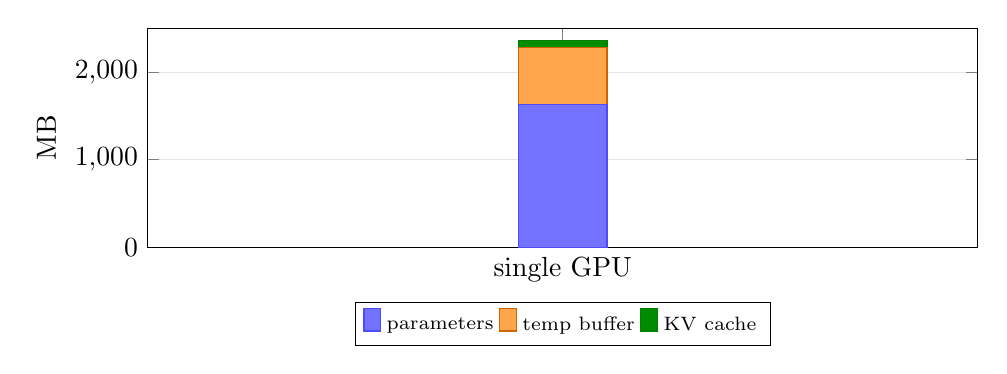
\begin{tikzpicture}
\begin{axis}[
    ybar stacked,
    width=\linewidth,
    height=0.36\linewidth,
    ymin=0,
    ymax=2500,
    ylabel={MB},
    symbolic x coords={single GPU},
    xtick=data,
    bar width=32pt,
    legend style={at={(0.5,-0.25)},anchor=north,legend columns=3,font=\scriptsize},
    grid=major,
    major grid style={draw=black!10},
]
\addplot+[fill=blue!55, draw=blue!70] coordinates {(single GPU,1626.943)};
\addplot+[fill=orange!70, draw=orange!80!black] coordinates {(single GPU,655.335)};
\addplot+[fill=green!55!black, draw=green!50!black] coordinates {(single GPU,75.150)};
\legend{parameters,temp buffer,KV cache}
\end{axis}
\end{tikzpicture}

  \caption{Estimated single-GPU memory components for the current compiled
  artifact.}
  \label{fig:memory}
\end{figure}

\section{Benchmark Methodology}

The benchmark prompt is ``What is in the image?'' on \texttt{kentucky.png},
with a 512 pixel fitted image size and 128 generated tokens. We report
generated tokens/s for end-to-end wrapper comparisons and effective decode
tokens/s for MLC when deferred CPU token commit would otherwise hide queued GPU
work outside the inner decode timer. The wrappers reject image-grid mismatches
and generated-token mismatches by default.

\begin{table}[t]
  \centering
  \caption{Current parity result on the batch-1 image benchmark.}
  \label{tab:parity}
  \begin{tabular}{lrr}
    \toprule
    Runtime & Generated tokens/s & Effective decode tokens/s \\
    \midrule
    MLC LLM & 414.23 & 446.09 \\
    vLLM & 413.30 & -- \\
    Transformers & 65.08 & -- \\
    \bottomrule
  \end{tabular}
\end{table}

\begin{figure}[t]
  \centering
  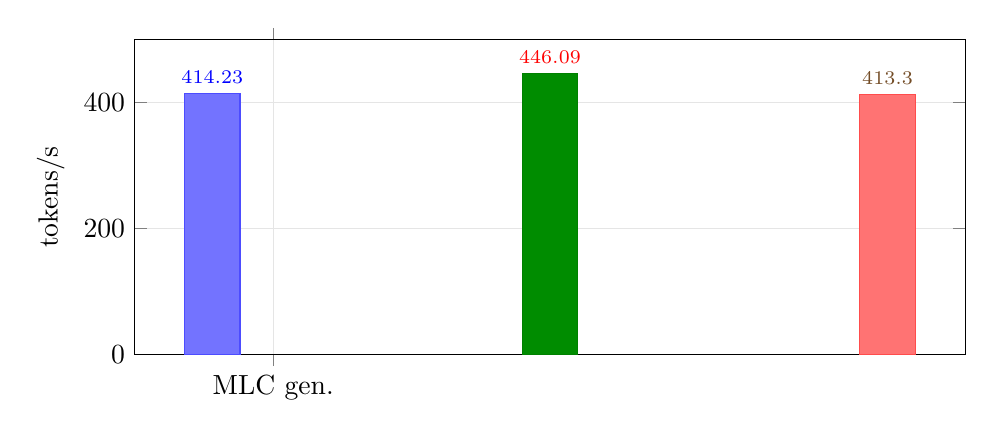
\begin{tikzpicture}
\begin{axis}[
    ybar,
    width=\linewidth,
    height=0.46\linewidth,
    ymin=0,
    ymax=500,
    ylabel={tokens/s},
    symbolic x coords={MLC gen.,MLC decode,vLLM gen.},
    xtick=data,
    nodes near coords,
    nodes near coords align={vertical},
    bar width=20pt,
    enlarge x limits=0.25,
    grid=major,
    major grid style={draw=black!10},
    every node near coord/.append style={font=\scriptsize},
]
\addplot+[fill=blue!55, draw=blue!70] coordinates {(MLC gen.,414.23)};
\addplot+[fill=green!55!black, draw=green!50!black] coordinates {(MLC decode,446.09)};
\addplot+[fill=red!55, draw=red!70] coordinates {(vLLM gen.,413.30)};
\end{axis}
\end{tikzpicture}

  \caption{Current batch-1 parity result. The MLC generated-token metric is
  directly comparable to the vLLM generated-token metric; the effective decode
  metric additionally accounts for deferred token-commit synchronization.}
  \label{fig:throughput}
\end{figure}

\section{Performance Evolution}

Performance improved incrementally as correctness and runtime boundaries were
made explicit. Figure~\ref{fig:timeline} plots representative milestones:
packed Gated DeltaNet support, stable decode inputs, captured cross-attention,
captured append and metadata paths, and relaxed metadata analysis that merges
decode into one graph region.

\begin{figure}[t]
  \centering
  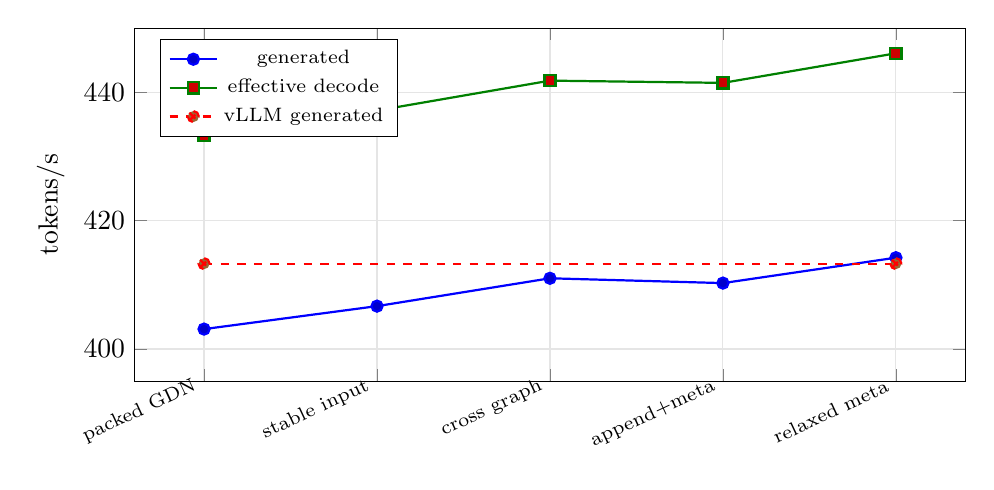
\begin{tikzpicture}
\begin{axis}[
    width=\linewidth,
    height=0.50\linewidth,
    ymin=395,
    ymax=450,
    ylabel={tokens/s},
    symbolic x coords={packed GDN,stable input,cross graph,append+meta,relaxed meta},
    xtick=data,
    x tick label style={rotate=25, anchor=east, font=\scriptsize},
    grid=major,
    major grid style={draw=black!10},
    legend style={at={(0.03,0.97)},anchor=north west,font=\scriptsize},
]
\addplot+[mark=*, thick, blue] coordinates {
    (packed GDN,403.10)
    (stable input,406.68)
    (cross graph,411.02)
    (append+meta,410.27)
    (relaxed meta,414.23)
};
\addlegendentry{generated}
\addplot+[mark=square*, thick, green!50!black] coordinates {
    (packed GDN,433.26)
    (stable input,437.17)
    (cross graph,441.83)
    (append+meta,441.48)
    (relaxed meta,446.09)
};
\addlegendentry{effective decode}
\addplot+[red, dashed, thick] coordinates {
    (packed GDN,413.30)
    (relaxed meta,413.30)
};
\addlegendentry{vLLM generated}
\end{axis}
\end{tikzpicture}

  \caption{Representative performance progression across implementation
  milestones. The vLLM generated-token line is included as the target baseline.}
  \label{fig:timeline}
\end{figure}

\begin{table}[t]
  \centering
  \caption{Selected implementation milestones.}
  \label{tab:milestones}
  \begin{tabular}{lll}
    \toprule
    Milestone & MLC gen. tok/s & Effective decode tok/s \\
    \midrule
    Packed GDN path & 403.10 & 433.26 \\
    Stable decode input & 406.68 & 437.17 \\
    Cross-attention graph capture & 411.02 & 441.83 \\
    Append and metadata capture & 410.27 & 441.48 \\
    Relaxed metadata tuple capture & 414.23 & 446.09 \\
    \bottomrule
  \end{tabular}
\end{table}

\section{Kernel Attribution}

Although this report is primarily about model support rather than low-level
kernel engineering, kernel attribution was necessary to determine whether
remaining performance differences came from runtime launch overhead or model
compute. A no-CUDA-graph diagnostic library was compiled so Nsight could see
internal decode kernels directly. The profile showed approximately 415 kernel
launches/token without graph capture and one graph replay/token in the
production artifact.

\begin{figure}[t]
  \centering
  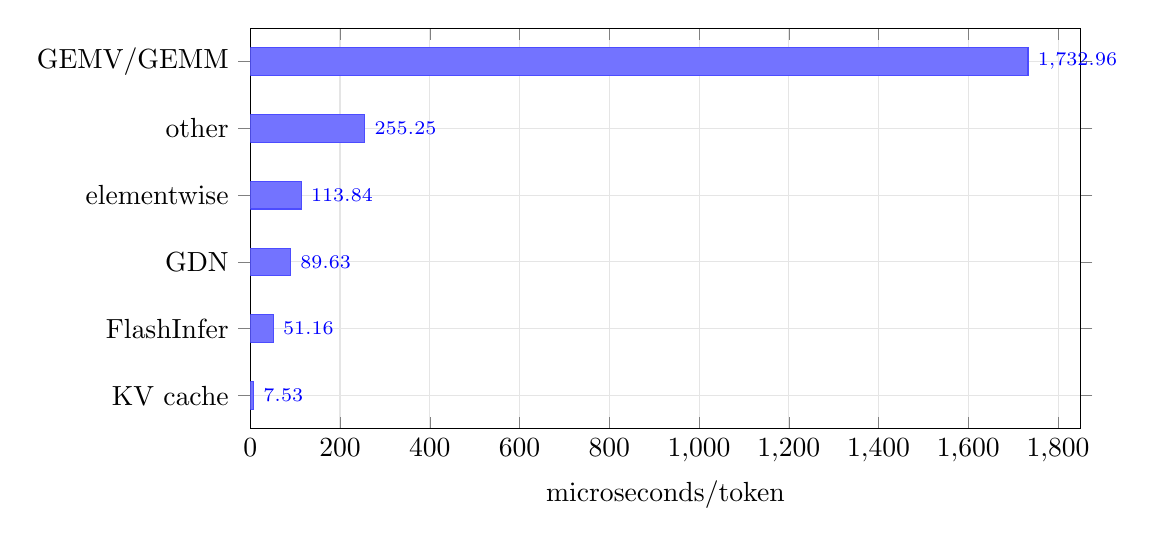
\begin{tikzpicture}
\begin{axis}[
    xbar,
    width=\linewidth,
    height=0.55\linewidth,
    xmin=0,
    xmax=1850,
    xlabel={microseconds/token},
    symbolic y coords={KV cache,FlashInfer,GDN,elementwise,other,GEMV/GEMM},
    ytick=data,
    nodes near coords,
    nodes near coords align={horizontal},
    every node near coord/.append style={font=\scriptsize},
    grid=major,
    major grid style={draw=black!10},
]
\addplot+[fill=blue!55, draw=blue!70] coordinates {
    (7.533,KV cache)
    (51.158,FlashInfer)
    (89.634,GDN)
    (113.838,elementwise)
    (255.254,other)
    (1732.960,GEMV/GEMM)
};
\end{axis}
\end{tikzpicture}

  \caption{No-graph decode attribution. GEMV/GEMM dominates the batch-1 decode
  profile, while FlashInfer attention is not the primary cost on this 2K-context
  workload.}
  \label{fig:kernel-breakdown}
\end{figure}

\begin{table}[t]
  \centering
  \caption{No-graph kernel-time attribution per decode token.}
  \label{tab:kernel-breakdown}
  \begin{tabular}{lrr}
    \toprule
    Category & Microseconds/token & Calls/token \\
    \midrule
    GEMV/GEMM & 1732.960 & 98.000 \\
    Other & 255.254 & 169.000 \\
    Elementwise & 113.838 & 112.000 \\
    GDN linear-attention & 89.634 & 18.000 \\
    FlashInfer attention & 51.158 & 12.000 \\
    KV cache & 7.533 & 6.000 \\
    \bottomrule
  \end{tabular}
\end{table}

The production graph-enabled profile exposed only one small query-position
preparation kernel at about 0.978 microseconds/token outside graph replay.
This supports the conclusion that the current artifact is already optimized at
the runtime-launch level; subsequent gains should come from higher-level model
or compiler specialization, not simply from adding another attention backend.

\section{Correctness and Validation}

Correctness validation focused on matching model semantics before comparing
speed. The support code includes tests for image-grid parsing, model path
resolution, vLLM tokenizer compatibility rewriting, benchmark output parsing,
subprocess failure handling, shell command syntax, Qwen3.5 model export,
KV-cache metadata behavior, and fixed-canvas image resize parity. The paper
package itself is generated from local artifacts and records the commands used
for benchmark reproduction.

\begin{table}[t]
  \centering
  \caption{Validation gates used during the implementation.}
  \label{tab:validation}
  \begin{tabular}{ll}
    \toprule
    Gate & Purpose \\
    \midrule
    \texttt{test\_qwen35.py} & Model export and Qwen3.5 frontend behavior \\
    \texttt{test\_qwen35\_benchmark\_wrapper.py} & MLC/vLLM wrapper parsing and parity checks \\
    \texttt{test\_compare\_nsys\_decode.py} & Nsight kernel/runtime categorization \\
    \texttt{bash -n} shell entrypoints & Quoting and semicolon-heavy compile options \\
    \texttt{check\_qwen35\_im\_parity.sh} & Transformers/MLC/vLLM image path parity \\
    \bottomrule
  \end{tabular}
\end{table}

\section{Lessons Learned}

\paragraph{Apples-to-apples benchmarking came first.}
Early comparisons were misleading until both paths used the same fine-tuned
checkpoint, image grid, generated-token count, and EOS behavior. The benchmark
wrapper's strict default checks were therefore as important as the model code.

\paragraph{Compiler wins depended on runtime contracts.}
CUDA graph capture improved only when the runtime state consumed by FlashInfer,
KV-cache metadata, and decode inputs became stable and explicit enough for the
compiler to reason about. Compiler analysis and runtime object design had to be
co-designed.

\paragraph{Attention was not the only question.}
Several attempts to swap or force attention backends produced smaller gains
than expected, and some fast microkernels did not improve whole-model decode.
The final result came from making the existing FlashInfer/cuBLAS path coherent
and graph-safe.

\paragraph{A compiled artifact is a product surface.}
The support work included tokenizer files, active vocabulary metadata, model
library naming, shell entrypoints, dry-run compile commands, diagnostic flags,
and vLLM-compatible checkpoint preparation. These details made the difference
between a one-off experiment and a reproducible deployment path.

\section{Limitations}

The evaluation is intentionally narrow. It uses one GPU, batch size 1, one
image, one prompt family, and one fine-tuned checkpoint. It does not evaluate
multi-request serving, long-context behavior beyond the compiled 2K window,
quantized accuracy/performance tradeoffs, mobile backends, or general
vision-language benchmarks. The reported parity should therefore be read as an
engineering result for a specific deployment target, not as a universal ranking
of inference systems.

\section{Conclusion}

We added MLC LLM support for a fine-tuned Qwen3.5 0.8B vision-language model
and brought the batch-1 image decode path to parity with a vLLM baseline on the
same checkpoint and image grid. The work required model frontend support,
vision preprocessing parity, Gated DeltaNet state handling, multimodal RoPE
support, weight conversion, explicit KV-cache metadata, CUDA graph capture, and
repeatable benchmarking. The outcome demonstrates that compiler-based LLM
deployment can support non-standard multimodal architectures, but also shows
that correctness, runtime contracts, and benchmark hygiene are prerequisites for
meaningful performance claims.

\bibliographystyle{plain}
\bibliography{references}

\end{document}
